% ---------------------------------------------------------------
% Generated by Flowchart -> TikZ Studio
% Every coordinate below is derived from the editor diagram model.
% Safe to edit by hand, but regenerating will overwrite changes.
% ---------------------------------------------------------------

\documentclass[border=8pt]{standalone}
\usepackage[T1]{fontenc}
\usepackage[utf8]{inputenc}
\usepackage{xcolor}
\usepackage{tikz}
\usetikzlibrary{arrows.meta,shadows,shapes.geometric,shapes.misc}

% ---- Colour definitions ----
\definecolor{fc0F9B8E}{HTML}{0F9B8E}
\definecolor{fc12161C}{HTML}{12161C}
\definecolor{fc1F2933}{HTML}{1F2933}
\definecolor{fc2F6FEB}{HTML}{2F6FEB}
\definecolor{fc7C8A9B}{HTML}{7C8A9B}
\definecolor{fcC65B3C}{HTML}{C65B3C}
\definecolor{fcD4F0EA}{HTML}{D4F0EA}
\definecolor{fcDBE8FF}{HTML}{DBE8FF}
\definecolor{fcE6EDF4}{HTML}{E6EDF4}
\definecolor{fcF7F9FB}{HTML}{F7F9FB}
\definecolor{fcFADFD8}{HTML}{FADFD8}

% ---- Style definitions ----
\tikzset{
  fcnode/.style={
    draw, inner sep=0pt, outer sep=0pt, align=center,
    line join=round, line cap=butt
  },
  fcpath/.style={line join=round, line cap=butt},
  fcedge/.style={line join=round, line cap=butt},
  fclabel/.style={inner sep=1.4pt, outer sep=0pt, align=center},
}

\begin{document}
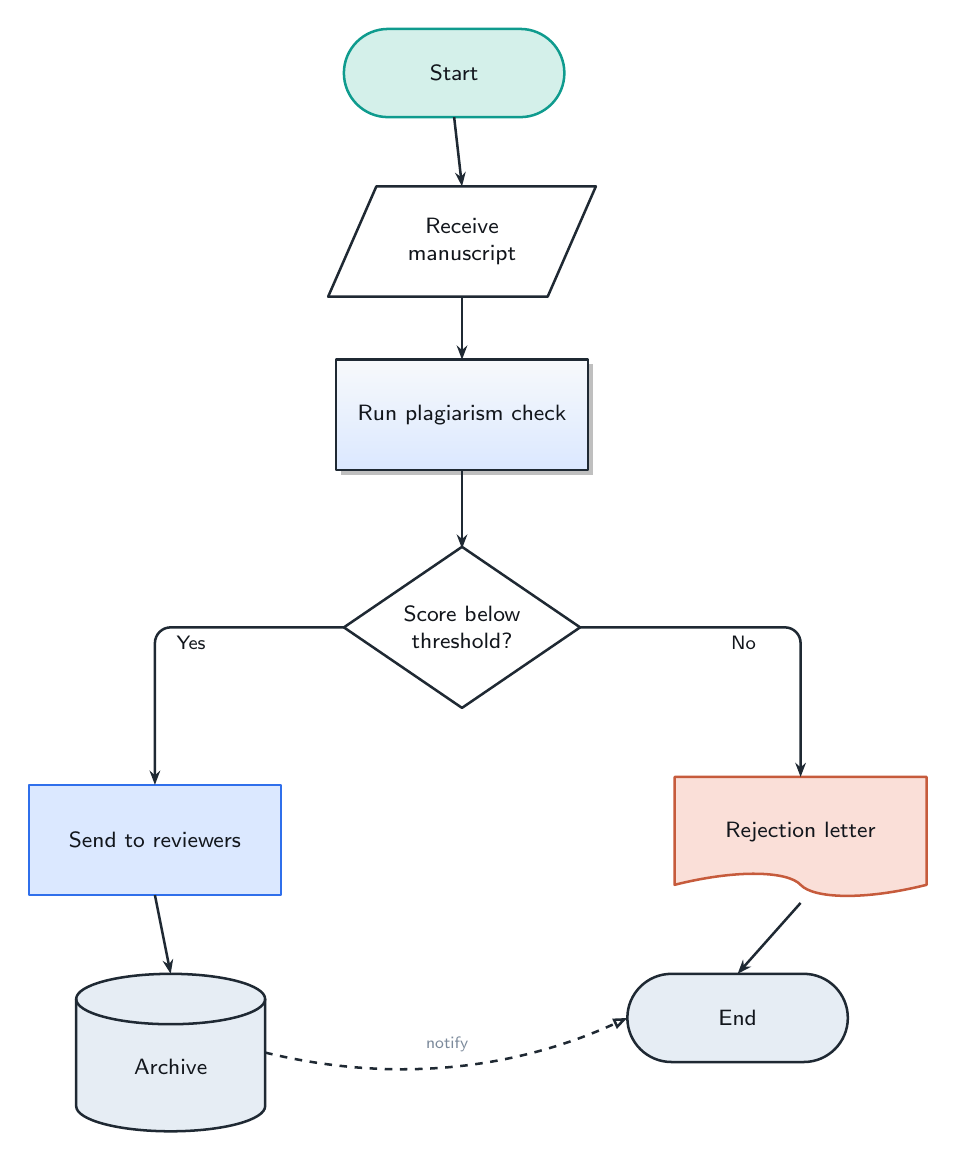
\begin{tikzpicture}[x=1cm, y=1cm]
  % ---- Nodes ----
  % n1 - Start / End "Start"
  \node[fcnode, shape=rounded rectangle, minimum width=2.8cm, minimum height=1.12cm,
        rounded rectangle arc length=180, draw=fc0F9B8E, line width=0.91pt, fill=fcD4F0EA,
        font=\fontsize{7.97pt}{9.96pt}\selectfont\sffamily, text=fc12161C, align=center,
        text width=2.128cm] (n1) at (6.6,-1.36) {Start};
  % n2 - Input / Output "Receive manuscript"
  \draw[fcpath, draw=fc1F2933, line width=0.91pt, fill=white]
    (5.612,-2.8) -- (8.4,-2.8) -- (7.788,-4.2) -- (5,-4.2) -- cycle;
  \coordinate (n2) at (6.7,-3.5);
  \node[fclabel, anchor=center, font=\fontsize{7.97pt}{9.96pt}\selectfont\sffamily,
        text=fc12161C, align=center, text width=2.04cm] at (6.7,-3.5) {Receive manuscript};
  % n3 - Process "Run plagiarism check"
  \node[fcnode, shape=rectangle, minimum width=3.2cm, minimum height=1.4cm, draw=fc1F2933,
        line width=0.91pt, top color=fcF7F9FB, bottom color=fcDBE8FF,
        drop shadow={shadow xshift=1.707pt, shadow yshift=-1.707pt, opacity=0.25, fill=black},
        font=\fontsize{7.97pt}{9.96pt}\selectfont\sffamily, text=fc12161C, align=center,
        text width=2.88cm] (n3) at (6.7,-5.7) {Run plagiarism check};
  % n4 - Decision "Score below"
  \node[fcnode, shape=diamond, minimum width=3cm, minimum height=2cm, draw=fc1F2933,
        line width=0.91pt, fill=white, font=\fontsize{7.97pt}{9.96pt}\selectfont\sffamily,
        text=fc12161C, align=center, text width=1.5cm]
        (n4) at (6.7,-8.4) {Score below \\ threshold?};
  % n5 - Process "Send to reviewers"
  \node[fcnode, shape=rectangle, minimum width=3.2cm, minimum height=1.4cm, draw=fc2F6FEB,
        line width=0.91pt, fill=fcDBE8FF, font=\fontsize{7.97pt}{9.96pt}\selectfont\sffamily,
        text=fc12161C, align=center, text width=2.88cm]
        (n5) at (2.8,-11.1) {Send to reviewers};
  % n6 - Document "Rejection letter"
  \draw[fcpath, draw=fcC65B3C, line width=0.91pt, fill=fcFADFD8]
    (9.4,-10.3) -- (12.6,-10.3) -- (12.6,-11.6696)
    .. controls (11.8,-11.8712) and (11.16,-11.8424) .. (11,-11.6696)
    .. controls (10.84,-11.4968) and (10.2,-11.468) .. (9.4,-11.6696) -- cycle;
  \coordinate (n6) at (11,-11.1);
  \node[fclabel, anchor=center, font=\fontsize{7.97pt}{9.96pt}\selectfont\sffamily,
        text=fc12161C, align=center, text width=2.88cm] at (11,-10.996) {Rejection letter};
  % n7 - Database "Archive"
  \draw[fcpath, draw=fc1F2933, line width=0.91pt, fill=fcE6EDF4]
    (1.8,-13.12) .. controls (1.8,-12.9433) and (2.3372,-12.8) .. (3,-12.8)
    .. controls (3.6628,-12.8) and (4.2,-12.9433) .. (4.2,-13.12) -- (4.2,-14.48)
    .. controls (4.2,-14.6567) and (3.6628,-14.8) .. (3,-14.8)
    .. controls (2.3372,-14.8) and (1.8,-14.6567) .. (1.8,-14.48) -- cycle;
  \draw[fcpath, draw=fc1F2933, line width=0.91pt]
    (1.8,-13.12) .. controls (1.8,-13.2967) and (2.3372,-13.44) .. (3,-13.44)
    .. controls (3.6628,-13.44) and (4.2,-13.2967) .. (4.2,-13.12);
  \coordinate (n7) at (3,-13.8);
  \node[fclabel, anchor=center, font=\fontsize{7.97pt}{9.96pt}\selectfont\sffamily,
        text=fc12161C, align=center, text width=2.08cm] at (3,-13.98) {Archive};
  % n8 - Start / End "End"
  \node[fcnode, shape=rounded rectangle, minimum width=2.8cm, minimum height=1.12cm,
        rounded rectangle arc length=180, draw=fc1F2933, line width=0.91pt, fill=fcE6EDF4,
        font=\fontsize{7.97pt}{9.96pt}\selectfont\sffamily, text=fc12161C, align=center,
        text width=2.128cm] (n8) at (10.2,-13.36) {End};
  % ---- Connectors ----
  % e1 - n1 -> n2 (straight)
  \draw[fcedge, -{Stealth[length=5.12pt, width=3.84pt]}, draw=fc1F2933, line width=0.91pt]
    (6.6,-1.92) -- (6.7,-2.8);
  % e2 - n2 -> n3 (straight)
  \draw[fcedge, -{Stealth[length=5.12pt, width=3.84pt]}, draw=fc1F2933, line width=0.91pt]
    (6.7,-4.2) -- (6.7,-5);
  % e3 - n3 -> n4 (straight)
  \draw[fcedge, -{Stealth[length=5.12pt, width=3.84pt]}, draw=fc1F2933, line width=0.91pt]
    (6.7,-6.4) -- (6.7,-7.4);
  % e4 - n4 -> n5 (rounded-orthogonal)
  \draw[fcedge, -{Stealth[length=5.12pt, width=3.84pt]}, draw=fc1F2933, line width=0.91pt]
    (5.2,-8.4) -- (4.96,-8.4) .. controls (4.8495,-8.4) and (4.6705,-8.4) .. (4.56,-8.4)
    -- (3,-8.4) .. controls (2.8895,-8.4) and (2.8,-8.4895) .. (2.8,-8.6) -- (2.8,-9.76)
    .. controls (2.8,-9.8705) and (2.8,-10.0495) .. (2.8,-10.16) -- (2.8,-10.4);
  \node[fclabel, anchor=center, font=\fontsize{6.83pt}{8.19pt}\selectfont\sffamily,
        text=fc12161C, fill=white, inner sep=1.6pt] (e4label) at (3.2586,-8.6) {Yes};
  % e5 - n4 -> n6 (rounded-orthogonal)
  \draw[fcedge, -{Stealth[length=5.12pt, width=3.84pt]}, draw=fc1F2933, line width=0.91pt]
    (8.2,-8.4) -- (8.44,-8.4) .. controls (8.5505,-8.4) and (8.7295,-8.4) .. (8.84,-8.4)
    -- (10.8,-8.4) .. controls (10.9105,-8.4) and (11,-8.4895) .. (11,-8.6) -- (11,-9.66)
    .. controls (11,-9.7705) and (11,-9.9495) .. (11,-10.06) -- (11,-10.3);
  \node[fclabel, anchor=center, font=\fontsize{6.83pt}{8.19pt}\selectfont\sffamily,
        text=fc12161C, fill=white, inner sep=1.6pt] (e5label) at (10.2764,-8.6) {No};
  % e6 - n5 -> n7 (straight)
  \draw[fcedge, -{Stealth[length=5.12pt, width=3.84pt]}, draw=fc1F2933, line width=0.91pt]
    (2.8,-11.8) -- (3,-12.8);
  % e7 - n6 -> n8 (straight)
  \draw[fcedge, -{Stealth[length=5.12pt, width=3.84pt]}, draw=fc1F2933, line width=0.91pt]
    (11,-11.9) -- (10.2,-12.8);
  % e8 - n7 -> n8 (curved)
  \draw[fcedge, -{Triangle[open, length=5.12pt, width=3.84pt]}, draw=fc1F2933,
        line width=0.91pt, dash pattern=on 2.731pt off 2.731pt]
    (4.2,-13.8) .. controls (5.7841,-14.1842) and (7.3174,-14.0376) .. (8.8,-13.36);
  \node[fclabel, anchor=center, font=\fontsize{6.26pt}{7.51pt}\selectfont\sffamily,
        text=fc7C8A9B] (e8label) at (6.5114,-13.6995) {notify};
\end{tikzpicture}
\end{document}